\section{Projektarchitektur}
Um die Abh�ngigkeitsverwaltung und das Bauen des Projektes m�glichst simpel zu gestalten, wurde f�r das Projekt Apache Maven \cite{maven} genutzt und das Projekt dementsprechend als Maven Projekt erstellt. \newline
Abh�ngigkeiten des Projekts sind der Amazon Kinesis Client in der Version 1.6.1, der Amazon Kinesis Producer in der Version 0.10.2 sowie Eclipse Jetty Servlet \cite{jetty} in der Version 9.2.14.v20151106. \newline
Die Projektarchitektur ist im Grunde genommen genau so, wie sie von Amazon in der Dokumentation von AWS Kinesis vorgestellt wird.

\begin{figure}[!h]

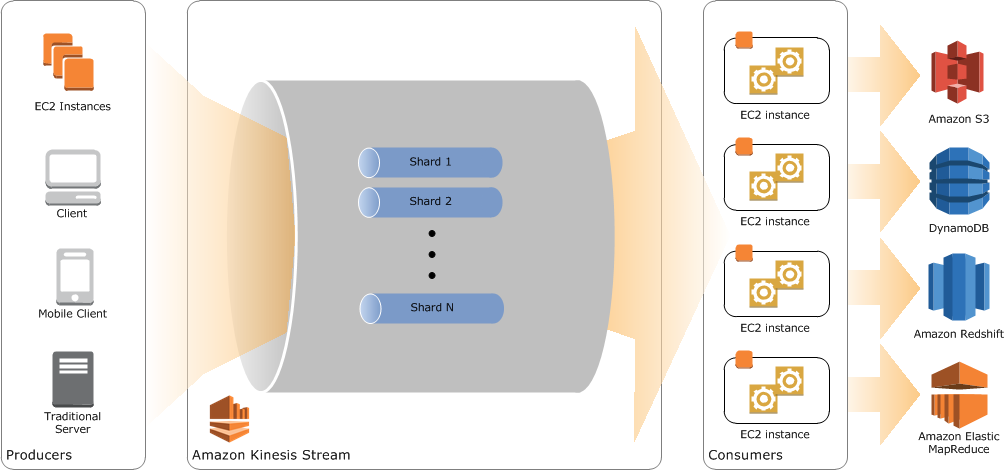
\includegraphics[width=1.0\textwidth]{content/images/kinesis_architecture.png}

\caption{Kinesis Architektur, wie sie von Amazon vorgegeben wird. Quelle: \cite{kinesis_concepts}}

\label{fig:aws_architecture}

\end{figure}

Wie in Abbildung. \ref{fig:aws_architecture} zu sehen, setzt Amazon in der Architektur 4 Schichten voraus. Die Producer, den Kinesis Stream, die Consumer sowie weitere Services au�erhalb von Kinesis. Die Daten werden von links nach rechts in der Architektur �bertragen. Zun�chst einmal werden die Daten in den Producern erzeugt und in den Kinesis Stream geschrieben, in denen sie in einem oder mehreren Shards einige Tage gespeichert bleiben. Ein Shard ist eine Gruppe von Datens�tzen in einem Kinesis Stream, die eine feste Menge an Daten aufnehmen k�nnen. \newline
Auf der anderen Seite des Kinesis Streams befinden sich ein oder mehrere Consumer, die die Daten aus den Shards des Kinesis Streams lesen. Nach dem Lesen k�nnen die Daten zudem an andere Services weitergeleitet werden, wie beispielsweise Amazon DynamoDB, mit dem die Daten in der NoSQL-Datenbank von DynamoDB persistiert werden k�nnen. \newline
Genau diese Architektur wurde auch im Projekt umgesetzt. Es gibt eine oder mehrere Instanzen des Producers, der Temperaturdaten erzeugt. Der Producer schreibt die Daten in einen Kinesis Stream, meist nur mit einem Shard, da ein Shard f�r die Datenmengen dieses Projekts ausreicht. Zudem gibt es eine oder mehrere Instanzen eines Consumers, der die Daten aus dem Kinesis Stream liest und dann in eine DynamoDB Datenbank schreibt. Dar�ber hinaus enth�lt dieses Projekt zudem eine Webapplikation, die die Temperaturdaten aus DynamoDB liest und in Diagrammen ausgibt. \newline
Zudem enth�lt das Projekt Utility-Klassen f�r DynamoDB, Kinesis sowie zur Temperaturgenerierung, in denen Methoden f�r die entsprechenden Anforderungsgebiete ausgelagert wurden. Dar�ber hinaus enth�lt das Projekt eine "DeleteResources" Klasse, die eine Methode zur L�schung aller verwendeten Ressourcen auf Amazon Webservices bereitstellt. \newline
In der pom.xml des Projekts sind mehrere Profile eingetragen, die es erm�glichen, einzelne Klassen mit Startparametern auszuf�hren um somit beispielsweise den Producer mit anderen Parametern zu starten (siehe Kapitel \ref{producer}).

\section{Producer}
\label{producer}

\section{Consumer}

\section{Webapplikation}

\section{L�schung der AWS Ressourcen}

Eine weitere Klasse ist die Klasse "DeleteResources", mittels der man die gestarteten Ressourcen auf Amazon Webservices wieder l�schen kann, um keine weiteren Kosten zu verursachen. \newline
Die Klasse hat eine main Methode, die zwei Argumente annimmt: Den Streamnamen sowie den Datenbank Namen der Dynamo DB Tabelle.
\lstinputlisting[firstline=24, lastline=30, caption=DeleteResources.java (24-30): Auslesen der �bergebenen Argumente, label=deleteresources_init_variables, style=java]{content/listings/DeleteResources.java}
In Quelltext \ref{deleteresources_init_variables} sieht man, wie die Argumente ausgelesen und gesetzt werden. Wenn nicht genau 2 Argumente �bergeben werden, wird ein Standardwert f�r die beiden Variablen genutzt. 
\lstinputlisting[firstline=32, lastline=43, caption=DeleteResources.java (32-43): Initialisierung der Dynamo DB Utilklasse und L�schen der Tabellen, label=deleteresources_init_db, style=java]{content/listings/DeleteResources.java}
In Quelltext \ref{deleteresources_init_db} wird die DynamoDB Utilklasse initalisiert und dazu werden zun�chst die ben�tigten Amazon Client Klassen erzeugt, die der Utilklasse bei der Initialisierung �bergeben werden. Daraufhin wird die �bersichtstabelle sowie die Tabelle, die die Temperaturdaten enth�lt, gel�scht.
\lstinputlisting[firstline=45, lastline=49, caption=DeleteResources.java: Initialisierung der Stream Utilklasse und L�schen des Streams (45-49), label=deleteresources_init_stream, style=java]{content/listings/DeleteResources.java}
Im n�chsten Abschnitt in Quelltext \ref{deleteresources_init_stream} wird dann die Stream Utilklasse initialisiert und daraufhin der Stream gel�scht. \newline
Damit sind alle Ressourcen, die auf Amazon Web Services genutzt wurden, gel�scht und es werden keine Kosten mehr zum Beispiel durch die tempor�re Speicherung der Daten im Kinesis Stream verursacht.
\section{Docker}

\section{Abweichungen im Vergleich zur Projektplanung}